\documentclass[12pt,a4paper]{amsart}

\usepackage[english]{babel}

\usepackage{amssymb,amsmath,amsfonts,amsthm}
\usepackage{graphicx}
\graphicspath{{./figures/}}
\usepackage[left=1in,right=1in,top=1in,bottom=1in]{geometry}

% Bibliography Style:
\usepackage[sort&compress,round]{natbib}
\setlength{\bibsep}{1ex}
\setlength{\bibhang}{1cm}

%\renewcommand{\baselinestretch}{2.0}

\usepackage{hyperref,url}
%\usepackage{pstricks,pst-node,pst-tree}

%\input xy
%\usepackage[cmtip]{xypic}
%\xyoption{all}
%\CompileMatrices

%\usepackage{newicktree}


\usepackage{array}


\newtheorem{thm}{Theorem}
\newtheorem{lemma}[thm]{Lemma}
\newtheorem{prop}[thm]{Proposition}
\newtheorem{cor}[thm]{Corollary}
\newtheorem{prob}[thm]{Problem}
\newtheorem{conj}[thm]{Conjecture}
\newtheorem{alg}[thm]{Algorithm}
\newtheorem{rmk}[thm]{Remark}

\newtheorem{ex}[thm]{Example}
\newtheorem{df}[thm]{Definition}

\newcommand{\eps}{\varepsilon}
\newcommand{\cE}{\mathcal{E}}
\newcommand{\cG}{\mathcal{G}}
\newcommand{\NN}{\mathbb{N}}
\newcommand{\RR}{\mathbb{R}}

\newcommand{\cA}{\mathcal{A}}
\newcommand{\cC}{\mathcal{C}}
\newcommand{\cS}{\mathcal{S}}
\newcommand{\cX}{\mathcal{X}}
\newcommand{\cY}{\mathcal{Y}}
\newcommand{\cZ}{\mathcal{Z}}
\newcommand{\Data}{\mathcal{D}}
\newcommand{\indep}{\perp}

\DeclareMathOperator{\pa}{pa}
\DeclareMathOperator{\E}{E}
\DeclareMathOperator{\Var}{Var}
\DeclareMathOperator{\Cov}{Cov}

\DeclareMathOperator{\HW}{HW}
\DeclareMathOperator{\Norm}{Norm}
\DeclareMathOperator{\Bern}{Bern}
\DeclareMathOperator{\Binom}{Binom}
\DeclareMathOperator{\Bernoulli}{Bernoulli}
\DeclareMathOperator{\Mult}{Mult}
\DeclareMathOperator{\Dir}{Dir}
\DeclareMathOperator{\Exp}{Exp}
\DeclareMathOperator{\Exit}{Exit}
\DeclareMathOperator{\Pois}{Pois}
\DeclareMathOperator{\MC}{MC}
\DeclareMathOperator{\Model}{M}
\DeclareMathOperator{\pos}{pos}
\DeclareMathOperator{\nt}{nt}


% For editing:
\usepackage{lineno}
\usepackage{color}
\newcommand{\niko}{\textcolor{red}}
\usepackage[colorinlistoftodos]{todonotes} 

\begin{document}

%\linenumbers
%\modulolinenumbers[2]

\title{A probabilistic model for reconstructing intra-tumor phylogenies}



\author{
NB-lab + FM-lab
}

\date{\today}

\begin{abstract}
We present an intra-tumor oncogenetic tree (ITOT) model for inferring tumor evolutionary histories from NGS data obtained from bulk sequencing of mixed tumor samples.
%We extend phylogenetic methods to infer cancer evolutionary trees from deep-sequencing data. 
Our methods not only infer the number of clones per sample but also the most likely life history of the tumor.
Our methods allow us to (i)~infer early events in tumour development, (ii)~link cancer heterogeneity to clinical outcome, (iii)~compare clonal evolution in metastasis to evolution in the primary tumour.
\end{abstract}


\maketitle


%%
%%
%%%%%%%%%%%%%%%%%%%%
%% INTRODUCTION
%%%%%%%%%%%%%%%%%%%%
%%
%%

\section{Introduction}

Cancers are heterogenous, the usual bla bla \cite{Shah2009,Nik-Zainal2012,Nik-Zainal2012a,Aparicio2013}

Progress has been made on clustering sequencing data into clonal subpopulations (\cite{Shah2012}, Ben Raphael's TheTA, Perou+Mardis paper soon), but the evolutionary relationships between these clones, the so called life history of a cancer, has so far only been estimated by eye \citep{Nik-Zainal2012a}. 

To change this sad situation, we need rigorous and accurate phylogenetic methods to automate the inference of the evolutionary history of a tumor. 
These methods will enable us to infer early driver events on a large scale, test whether evolutionary trajectories are predictive of outcome, and compare clonal evolution between pimary and metastatic tumors.
%The link between patient-specific clonal evolution and clinical outcomes like relapse or progression-free survival has not been rigorously tested. 
Better phylogenies will improve the usefulness of all cancer heterogeneity studies, which so far are limited to enumerating longer and longer lists of mutations and aberrations.
Our work extends methods proposed in \cite{Schwarz2013a,Schwarz2013b} from multiple-sampled copy-number profiles to SNVs from deep-sequencing data.

%We would like to reconstruct the evolutionary history of individual tumors. 
%Each tumor consists of multiple subclonal genetic variants that have evolved after its last clonal expansion. 
We assume that the mixed tumor cell population has been bulk sequenced, such that the resulting reads provide a statistical sample of the underlying population.
Ignoring structural variation and copy number alterations, we aim at inferring a phylogenetic tree model that represents the evolutionary history of the tumor clones from the observed short read data focusing only on single-nucleotide variations (SNVs). 
This task is different from classical phylogenetic approaches in at least three ways: 
(i) The observed data are short reads covering only a small fraction of the cancer genotypes that define the subclones. 
(ii) Due to the bulk sequencing approach of mixed samples, it is unknown which read originated from which cancer genotype. 
(iii) Read counts allow for inference of relative frequencies of mutations, which are informative about the order in which mutations have occurred.   

The starting point of our method development will be existing methods for estimating clonal populations. 
A prominent example is pyclone \citep{Shah2012}, which corrects mutation frequencies for copy number alterations and loss of heterozygosity and clusters the frequency distribution using a Dirichlet process mixture model. 
The outcome of this analysis is the number of clones and their frequencies; what is still unknown is the evolutionary history of the clones and previous approaches have relied on visual analysis to place clones in a phylogenetic tree \citep{Nik-Zainal2012a}. 

We will automate this process by implementing the key ideas of \citet{Nik-Zainal2012a}  in a rigorous statistical model. 
The central insight is that the way clonal frequencies add up hints at their evolutionary history. 
Figure~\ref{fig1}A illustrates this idea in an idealized scenario by showing how a population of three clones (with genotypes A, BC, BD) results in a mutation frequency distribution with four peaks (centred around the frequencies of A,B,C,D). 
The tree structure is reflected in the frequency distribution: frequencies of A and B add up to 100\% and frequencies of C and D add up to the frequency of B, their ancestor in the tree. \todo{this might be a bit too constrained} 
However, in noisy data these relationships can be blurred, which makes tree construction difficult. 
In particular, the clustering could result in spurious clusters or misplaced cluster centers that cannot be fit in a tree. 
This is the reason why in the manual reconstruction in \cite{Nik-Zainal2012a} one of the big clusters had to be split by hand into three smaller ones that were attached to different parts of the tree.

\begin{figure}[t]
\centerline{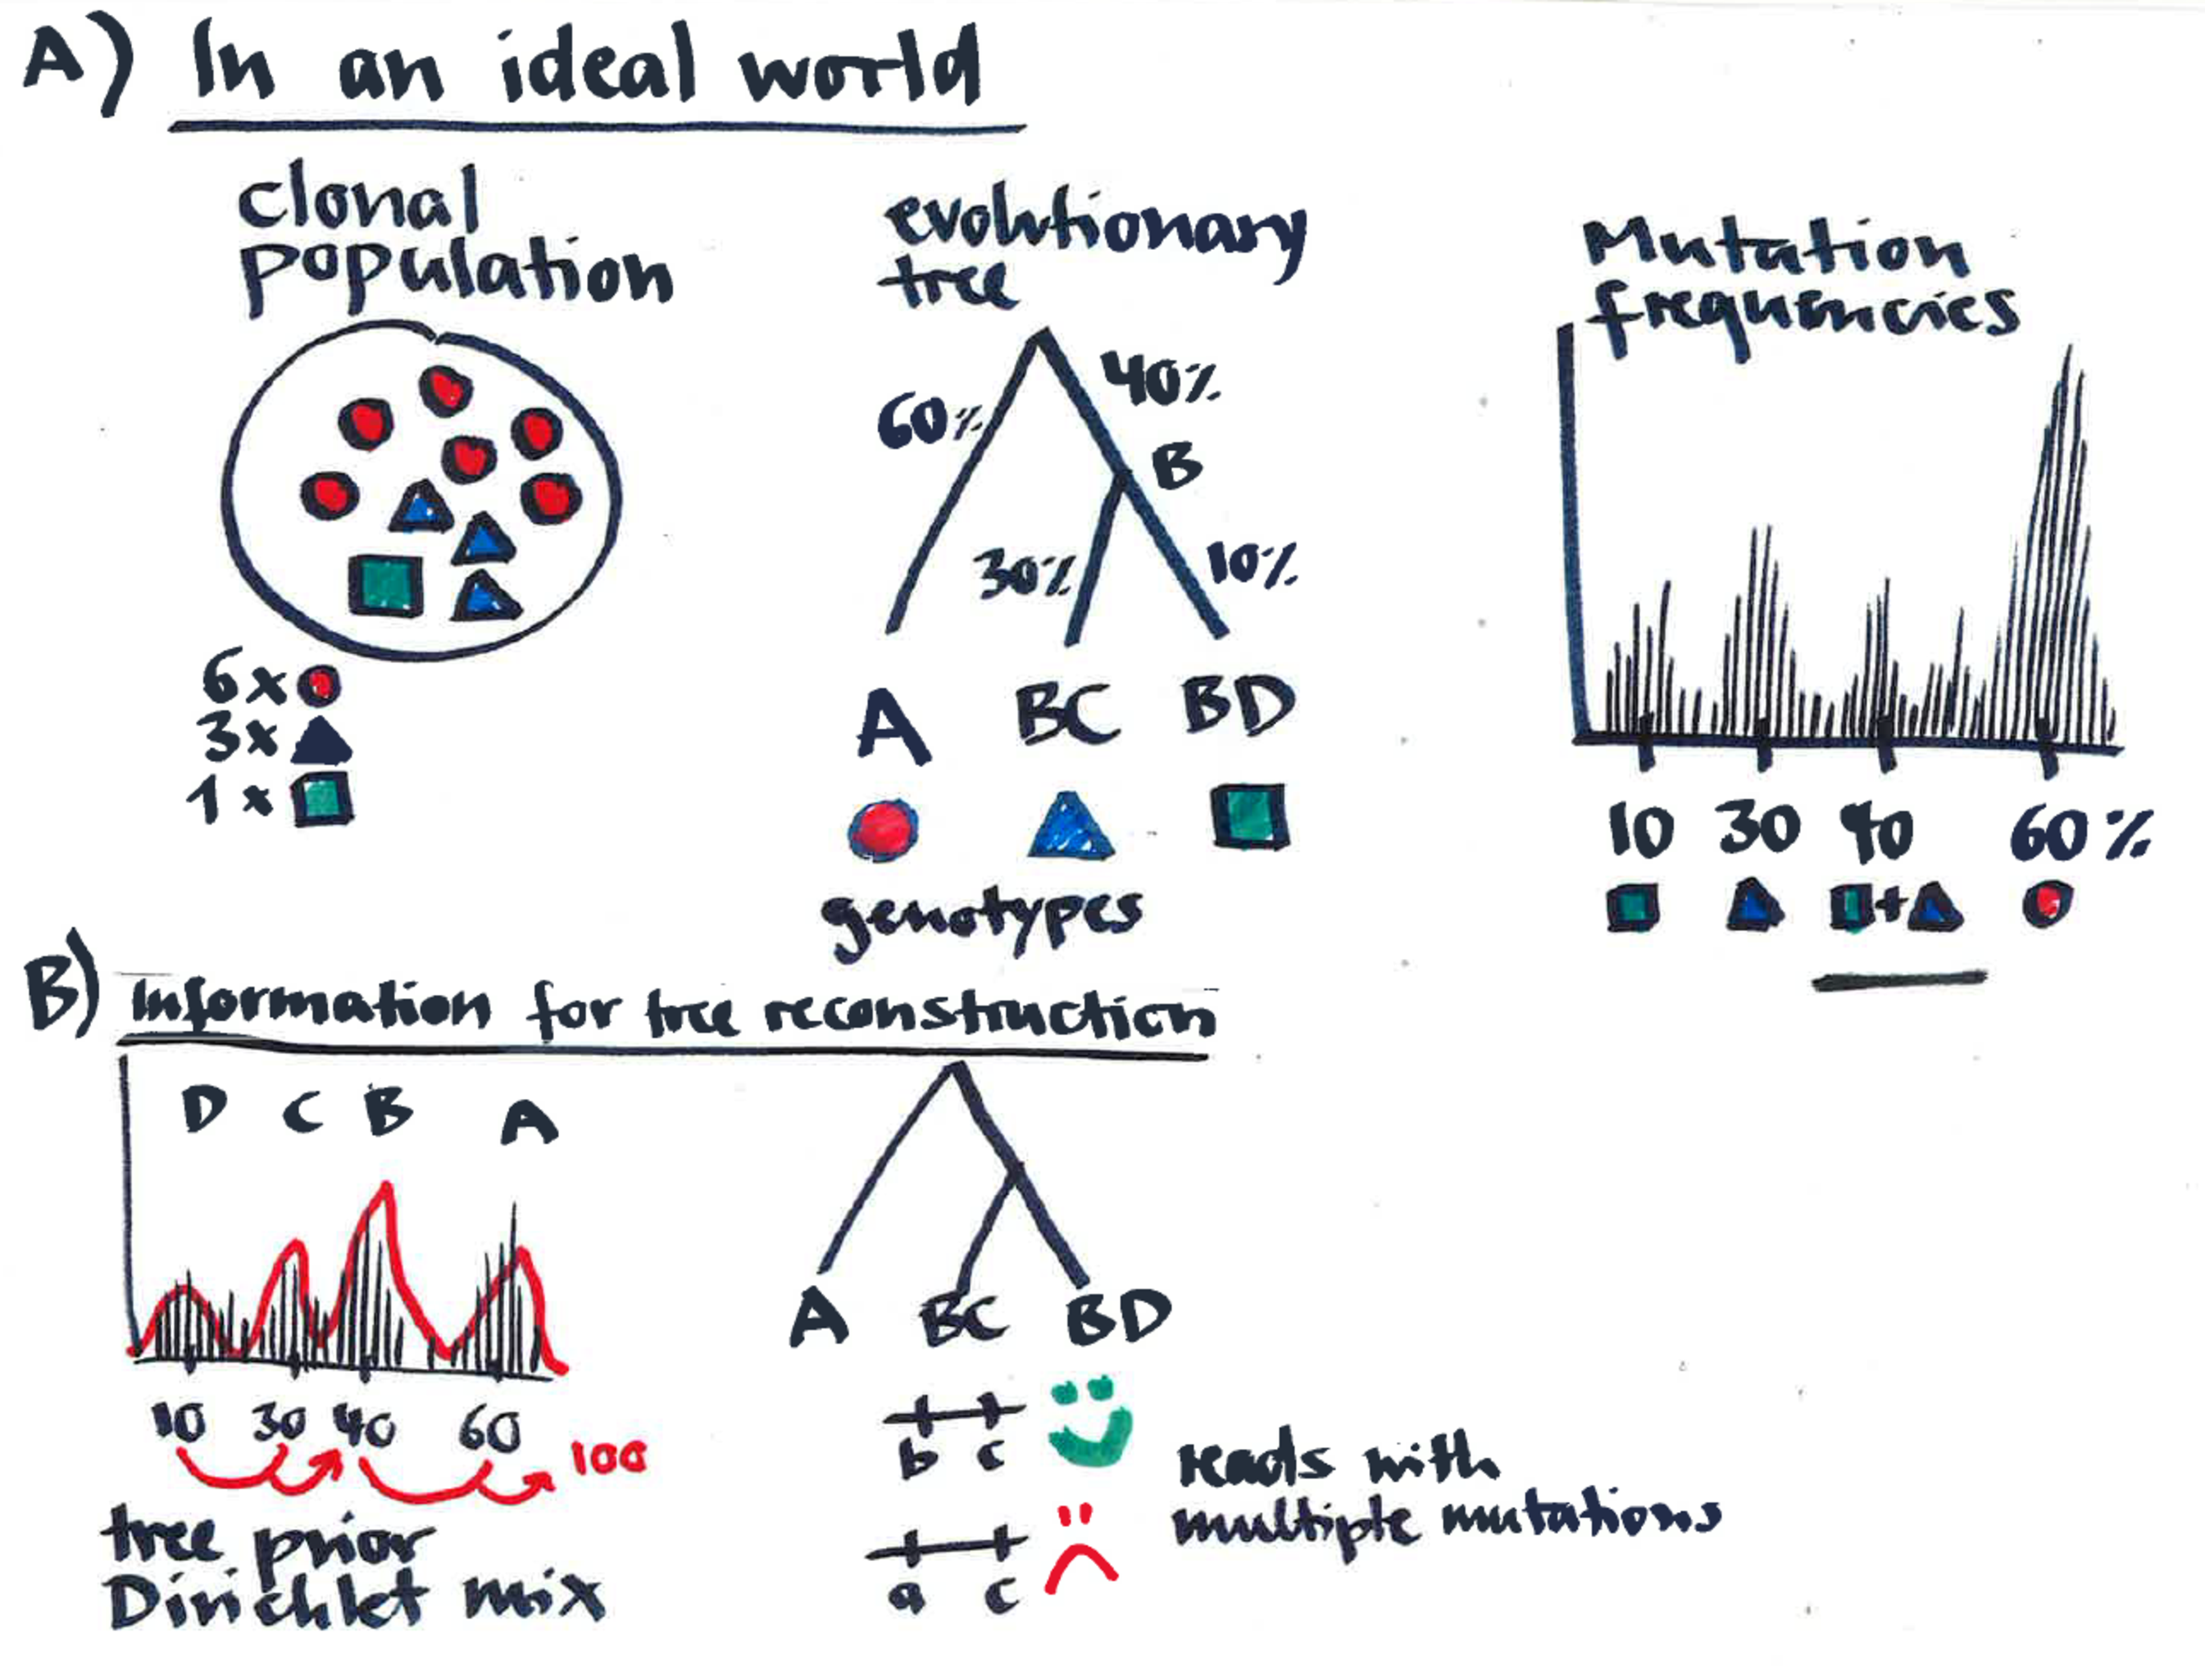
\includegraphics[width=.9\textwidth]{fig1}}
\caption{\textbf{A)} Overview how heterogeneity in a tumor relates to clonal evolution and is reflected in mutation frequencies. \textbf{B)} The sources of information we have available for inference.}
\label{fig1}
\end{figure}

To address these problems, we propose the following approach. 
We will start by calling mutations from deep-sequencing data and correcting their frequencies for copy-number and loss of heterozygosity in the same way as pyClone. 
To infer clonal evolutionary trees we will use two complementary pieces of information (Figure~\ref{fig1}B): First, we will constrain the clustering of mutation frequencies to ensure that clonal frequencies are �tree-like�. 
Instead of sequentially clustering and tree-building we will combine both steps into a single model, following ideas of \citet{Adams2010,Williams1999}.
As a result our mixture model will automatically (1) estimate the number of clones and (2) place them in an evolutionary tree. 

A second source of information to validate this tree are the reads that contain more than one mutation. 
In the example of Figure~\ref{fig2} reads with mutations from both B and C would agree with the tree, but all reads with mutations from A and C would be evidence against it. 
Our final model will integrate the tree-constrained clustering with the information in multiply mutated reads into a joint likelihood to estimate the most likely tree topology.

\section{Our goals}

\begin{figure}[b]
\centerline{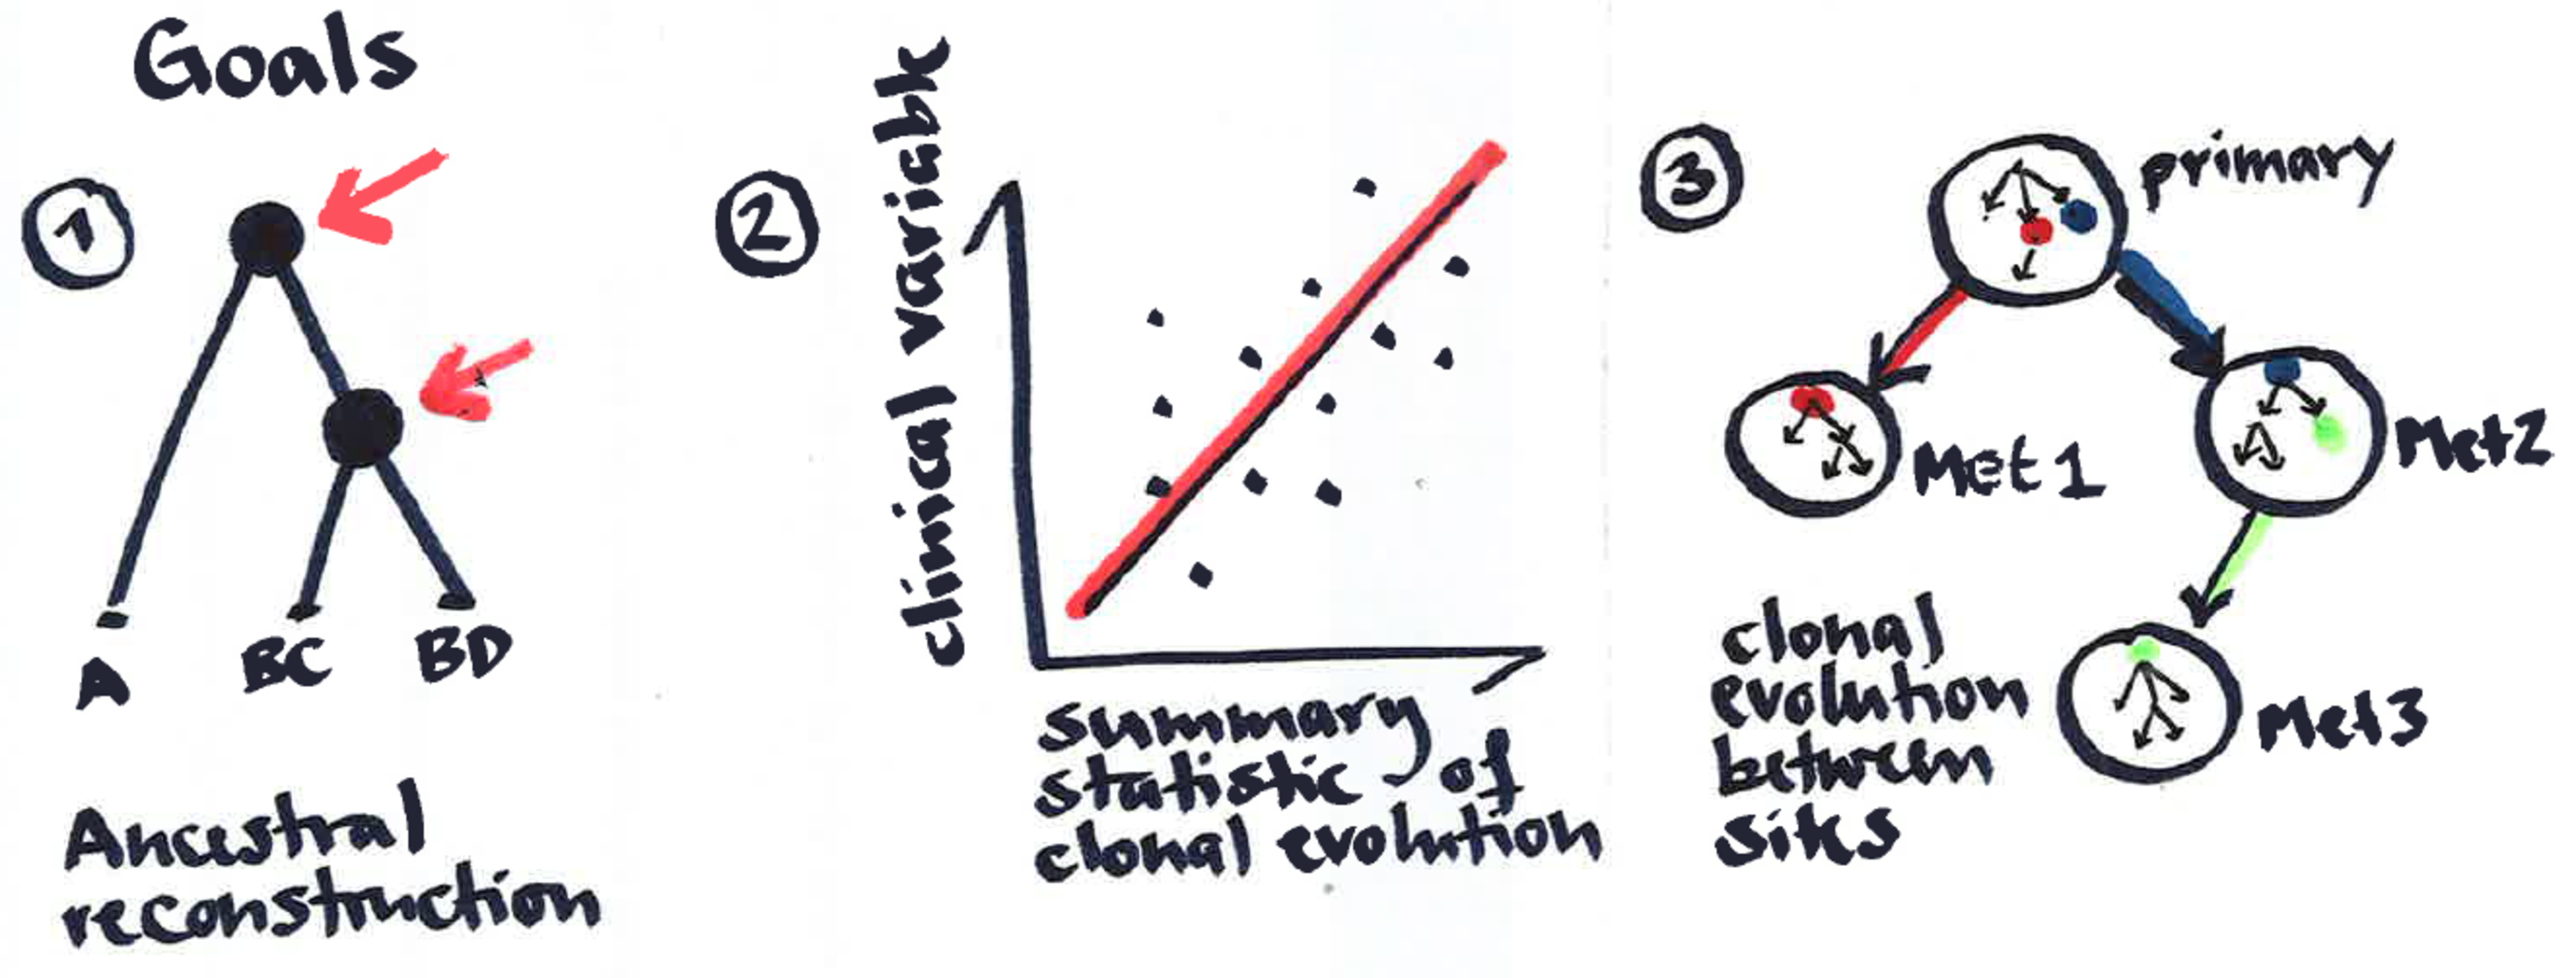
\includegraphics[width=.9\textwidth]{fig2}}
\caption{\textbf{Goals of our analysis are} (i)  to infer early events in tumour development, (ii) to link cancer heterogeneity to clinical outcome, (iii) to compare clonal evolution in metastasis to evolution in the primary tumour.}
\label{fig2}
\end{figure}


Our method will allow us to investigate three pivotal questions:

\subsection*{1. In which order did genomic events occur during tumor development?}
Earlier driver events will be more important drug targets than newer ones.
To time events, our first goal will be to automate the phylogenetic inference of clonal evolution, as exemplified in Nik-Zainal et al (2012).

We will validate our approach using simulations of tumour evolution driven by basic biological principles, following the ideas developed in \cite{Schwarz2013a}. 

This project will be our main focus in the beginning. Once the model is established, the next project is basically for free (except for the blood, sweat and tears of applying it).

\textbf{Data:} We will use the data of \citet{Nik-Zainal2012} to compare our automatically reconstructed trees to their visual analysis. \todo{Are there any other clonal trees out there that we could compare against?}

\subsection*{2. How predictive are �life histories� of tumours for clinical endpoints?}
In esophageal adenocarcinoma measures of clonal heterogeneity (entropy: number of clones weighted by their frequency) predict disease progression \citep{Maley2006}.
This is a landmark study, because the link between heterogeneity and clinical variables is still widely unexplored.
\citet{Maley2006} identified clones by any difference in flow cytometric DNA content (for differences 40.2N), LOH, microsatellite shifts (new alleles) and CDKN2A or TP53 sequence mutations.

We will extend the analysis of \citet{Maley2006} to deep sequencing data.
Using the trees from our method we will compute summary statistics that measure genomic heterogeneity of the tumor and quantify features of its evolutionary history. The simplest summary statistics (and baseline of our analysis) are the number of clones and entropy of their distribution \citep{Maley2006}, which do not take any features of the tree into account. Our hypothesis is that measures of heterogeneity, which explicitly rely on features of the tree structure, are more informative than the number of clones.

\textbf{Data:} We will apply our method to the 65 triple-negative breast cancers sequenced in \cite{Shah2012}, for which clinical data is available. \todo{We can already now conpute clonal distribution + entropy for all theses samples (as Shah et al have done already) and correlate with outcome.} We will also need a validation set of at least equal size.\todo{Where do we get this?} We can use all available data from all cancers. Being able to compare the predictive power of trees between cancer types would make us stronger. \todo{Collect all data!}
 
\subsection*{3. How does clonal evolution in the patient span primary tumour and metastases?}
In a (so far) unpublished project Elaine Mardis and Chuck Perou work on data of sequencing samples of a primary breast tumour and five metastases at different anatomical sites. They clustered sequencing data into clones individually for each sample and ordered the samples into a tree using Phylip on the average genomic profile. 

We will algorithmically improve this analysis by developing methods for joint inference of sample-specific trees and a global tree, which together will show how clones evolve within a tumor and spread to other anatomical sites to start a metastasis. This approach will �borrow information� across samples to identify small clonal subpopulations that might be missed if samples are treated independently.

The goal is to infer clonal evolution in the patient, spanning different anatomic sites and showing how clones move from one site to the next and populate a metastases.

\textbf{Data:} These data are not yet published, but Mardis is giving talks -- can't be long. It would be good to have a basic method ready when the data come out.

\section{How to get started}

\begin{itemize}
\item First step: during Thomas' visit we will start merging our methodological ideas (see below) and derive a battle plan for method development.
\item Repository for  code, manuscripts and data(?). Any objections to using bitbucket?
\item Data collection: these genetic data take a while to collect because of all the bureaucratic hoops to jump through. We need to start now basically even if we don't plan to touch them for months.
\item Regular meetings. Every two weeks?
\end{itemize}


%%
%%
%%%%%%%%%%%%%%%%%%%%
%% METHODS
%%%%%%%%%%%%%%%%%%%%
%%
%%

\section{Methods (Basel)}

An SNV $x$ is defined by its genomic position $\pos(x)$ and its variant nucleotide $\nt(x) \in \cA := \{{\tt A,C,G,T}\}$.
Let $\cS$ denote the set of all SNVs in a given tumor.
NGS of the tumor produces short reads and we consider only those reads that overlap
with at least one segregating site $j \in \{\pos(x) \mid x \in \cS\}$.
We assume that each read contains either one or two SNVs (relative to the most frequent nucleotide at the respective position). Reads without SNVs are not informative and those with more than two SNVs are so rare that we can ignore them. 
Then the data $X$ consists of $N_1$ reads carrying one SNV, $x_1^{(i)} \in \cS$, $i=1,\dots,N_1$, and $N_2$ reads with
pairs of SNVs, $x_2^{(i)} \in \cS^2$, $i=1,\dots,N_2$. 

An intra-tumor oncogenetic tree (ITOT) is a labeled binary rooted tree $T = (V, E, r, g, f, s)$ (Figure~\ref{fig:tree}).
The edges $e \in E$ are labeled with sets of SNVs, $s : E \to 2^{\cS}$, that have occurred on this branch
such that they define a partition of the set of all SNVs, i.e., $s(e_1) \cap s(e_2) = \emptyset$ for all edges
$e_1 \not= e_2$ and $\cup_{e \in E} s(e) = \cS$.  
The vertices $v \in V$ represent subclones and are labeled (uniquely) with genotypes. A genotype is a set of co-ocurring SNVs and each vertex is labeled by the set of all SNVs that have given rise to it. Formally, let $(e_1, \dots, e_M)$ be the unique path (ordered set of edges) connecting the root vertex $r$ with vertex $v \in V$. Then the genotype label $g : V \to 2^{\cS}$ of vertex $v$ is $g(v) = \cup_{m=1}^M s(e_m)$.
It follows that $g(v) = g(w_1) \cap g(w_2)$ for all branching points $v$ into daughter clones $w_1$ and $w_2$. 
The root of the tree is the genotype after the last clonal expansion of the tumor, the leaves of the tree are the subclones at the time of observation (diagnosis), and the interior vertices are extinct common ancestor clones. We denote by $L \subset V$ the set of leaves (contemporary clones). 
In addition, vertices are labeled with their relative frequencies within the tumor, $f : V \to (0,1]$,
subject to the following constraints: (i) $f(r) = 1$, (ii) $\sum_{v \in L} f(v) = 1$, and
(iii) $f(v) = f(w_1) + f(w_2)$ for all branching points $v$ into daughter clones $w_1$ and $w_2$.
Note that if (ii) holds for a function $f : L \to (0,1]$, then $f$ can always be extended in a unique way to $V$ 
such that (i) and (iii) also hold. 


\begin{figure}[t]
\flushleft
{\tt
~~----------- A ~~0.7\\
~|\\
-+ r\\        
~|~~~~~------ BC ~0.2\\
~~----+ B\\
~~~~~~~------ BD ~0.1\\
}
\caption{\label{fig:tree}
ITOT for three clones. Edges are labeled from top to bottom by
SNV sets A, C, B, D.  Vertices are labeled from top to bottom by
genotypes A (leaf), r (root), BC (leaf), B (internal), BD (leaf),
and by clone frequencies 0.7, 1.0, 0.2, 0.3, 0.1.
}
\end{figure}


The ITOT model consists of an ITOT $T = (V, E, r, g, f, s)$ for generating genotypes $G$ and a probabilistic model for generating reads, i.e., single SNVs $X_1$ and SNV pairs $X_2$, from genotypes.
Let $L = \{g_1, \dots, g_K\}$ denote the genotypes of the contemporary clones, i.e., the leaves of the tree.
Each leaf genotype $G$ is generated with probability
\begin{equation}
	\Pr(G = g_k) = f_k
\end{equation}
where $f_k \in (0,1]$ are parameters such that $\sum_{k=1}^K f_k = 1$. The parameters $f_k$ define
the clone frequencies of the ITOT via $f(g_k) = f_k$ and its unique recursive extension to $V$.
The conditional probabilities of observing single and pair SNVs are, respectively,
\begin{eqnarray}
	\Pr(X_1 = s \mid G = g) &=&
		\begin{cases}
			\eps   & \text{if $|\{s\} \cap g| = 0$} \\
     		1-\eps & \text{if $|\{s\} \cap g| = 1$}
		\end{cases} \\[1ex]
	\Pr(X_2 = (s,t) \mid G = g) &=&
		\begin{cases}
			\eps^2        & \text{if $|\{s,t\} \cap g| = 0$} \\
     		2\eps(1-\eps) & \text{if $|\{s,t\} \cap g| = 1$} \\
     		(1-\eps)^2    & \text{if $|\{s,t\} \cap g| = 2$}
		\end{cases}
\end{eqnarray}
where $\eps$ is the error probability accounting for misassignment of SNVs to their clones.
The ITOT model is the mixture model
\begin{eqnarray*}
	\Pr(X_m \mid T) &=& \sum_{k=1}^K \Pr(X_m, G = g_k) = \sum_{k=1}^K \Pr(X_m \mid G = g_k) \Pr(G = g_k),
	\quad m=1,2
\end{eqnarray*}

To learn the structure and parameters of the ITOT model for fixed $K$ from
observed SNV data, we devise a structural EM algorithm.
In the E step, we compute the responsibility of each leaf genotype
for each observed read. In the M step, we re-estimate the ITOT.


\subsection{E step}

The responsibility of leaf genotype $g_k$ for observation $x_m^{(i)}$,
$m=1,2$, $i=1,\dots,N_m$, is

\begin{eqnarray}
	\gamma_{mik} &:=& \Pr(G = g_k \mid X_m = x_m^{(i)})\\
	&=& \frac{\Pr(X_m = x_x^{(i)} \mid G = g_k) \Pr(G = g_k)}
		{\sum_{k=1}^K \Pr(X_m = x_x^{(i)} \mid G = g_k) \Pr(G = g_k)} 
\end{eqnarray} 


\subsection{M step}

The ML step consists of maximization over the discrete structures tree topologies
and SNV partitions, and over the continuous parameters $f$ (clone frequencies)
and $\eps$ (error probability). For given leaf genotypes $g_1, \dots, g_K$, the MLEs of $f$ and $\eps$ are, respectively,
\begin{eqnarray}
	\hat{f}_k &=& \frac{\sum_{m=1,2} \sum_{i=1}^{N_m} \gamma_{mik}}{N_1 + N_2},
		\quad k=1,\dots,K \\[1ex]
	\hat{\eps} &=& \frac{\sum_{m=1,2} \sum_{i=1}^{N_m} \gamma_{mik} (m - |x_m^{(i)} \cap g_k|)}{N_1 + 2N_2}
\end{eqnarray} 

Estimation of the leaf genotypes involves reconstruction of the ITOT from 
the responsibilities $\gamma_{mik}$. Exact ML estimation seems difficult, but we
can employ heuristics, such as distance-based phylogenetic methods.
The distance between clone $k$ and clone $l$ may be defined as
\begin{equation}
	d_{kl} = \sum_{m=1,2} \sum_{i=1}^{N_m} (1 - 2 \min\{\gamma_{mik}, \,\gamma_{mil}\})
\end{equation}
The resulting tree $(V, E)$ can be labeled recursively from the leaves to the
root by setting 
$g(g_k) = \cup_{m,\,i} \{x_m^{(i)} \mid \gamma_{mik} \geq \eta\}$
for all leaves $g_k$, and $g(v) = g(w_1) \cap g(w_2)$ for all branchings
$v$ into daughters $w_1$, $w_2$. 
Here, the paramter $\eta$ controls the multiple, hard assignment of SNVs to genotypes.
$\eta \approx \eps$ for single and $\eta \approx \eps^2$ for pairs of SNVs appears a reasonable choice, or else a preset fixed cutoff.

Alternatively, the triplet search may be employed here ...

From $g : V \to 2^{\cS}$, edge
labels $s : E \to 2^{\cS}$ can be inferred. Clone frequencies
$f$ can then be estimated for all leaves as described above and
extended to $V$ as described earlier. 

\section{Methods (Cambridge)}

to come

%%
%%
%%%%%%%%%%%%%%%%%%%%
%% RESULTS
%%%%%%%%%%%%%%%%%%%%
%%
%%

%\section{Results}


%\section{Discussion}




%%
%%
%%%%%%%%%%%%%%%%%%%%
%% REFERENCES
%%%%%%%%%%%%%%%%%%%%
%%
%%
\bibliographystyle{abbrvnat}
%\bibliography{./references/ITOT}
\bibliography{./ITOT}

%%
%%
%%%%%%%%%%%%%%%%%%%%
%% The end, my friend!
%%%%%%%%%%%%%%%%%%%%
%%
%%
\end{document}
